\documentclass{beamer} 
\usepackage{amsmath,amsthm}
\usepackage{mathrsfs}
\usepackage{amssymb}
\usepackage[english]{babel}
\usepackage{latexsym}
\usepackage{amsfonts}
\usepackage{graphicx}
\usepackage{float}
\usepackage{graphics}
\usepackage{epsfig}
\usepackage{url}
\usepackage{soul}
\usepackage{listings}
\usepackage{bm}
\usepackage{braket}

% \usepackage{minted}


\usetheme{WVU}
\usecolortheme{WVU}
\usepackage{multirow}

\mode<presentation> 

\title[VE401 SU2022 RC week12]{VE401 SU2022 RC week12 \& Onsite Evaluation}

\author[ Shuyu Wu ]{ Shuyu Wu }
\institute[UM-SJTU JI]{UM-SJTU Joint Institute \vspace{.2cm} \\ 
\includegraphics[scale=0.3]{umji_logo.png}\\wushuyu2002@sjtu.edu.cn}
\date[July 2022]{\today}

\begin{document}
\begin{frame} 

\titlepage 

\end{frame} 


\section{Short Recap: Multiple Linear Regression I: Basic Model}
\begin{frame}
    \frametitle{Outline}
    \tableofcontents[currentsection]
\end{frame}


\begin{frame}
    \frametitle{Generalized Regression Models}
    \begin{enumerate}
        \item Generalize the number of variables
        \[\mu_{Y|x_1\dots x_p}=\beta_0+\beta_1 x_1+\dots +\beta_p x_p\]
        \item Generalize the degree of the polynomial
        \[\mu_{Y|x}=\beta_0+\beta_1 x+\dots +\beta_p x^p\]
        \item Mixture, for example, 
        \[\mu_{Y|x_1\dots x_p}=\beta_0+\beta_1 x_1+\beta_2 x_2+\beta_3 x_1 x_2\]
    \end{enumerate}
    These are all called \textbf{Multiple Linear Regression}, and we have a set of general theory to tackle these problems.\par
    Question: Why 2 and 3 are also called ``linear''?
    

\end{frame}

\begin{frame}
    \frametitle{The Polynomial Model}

    We first talk about Polynomial Model.\par
    Suppose we have a set of n sample, $(x_i,y_i)$, $i=1,2,\dots , n$. Our goal is to find the estimate of $\beta_0$ to $\beta_p$, denoted as $b_0, \dots , b_p$, such that
    \[y_i=b_0+b_1 x_{i}^1+\dots +b_p x_i^p+e_i\]
    And the sum of squares error, 
    \[SS_{E}=\sum\limits_{i=1}^{n} e_i^2\]
    is minimized.

\end{frame}

\begin{frame}
    \frametitle{The Model Specification Matrix}

    For the model $Y_i=\beta_0+\beta_1 x_i+\dots +\beta_p x_i^p + E_i$, $i=1,2,\dots , n$, we can use a matrix equation to represent
    \[\mathbf{Y}=X\boldsymbol{\beta}+\mathbf{E}\]
    And 
    \begin{equation*}      
        \mathbf{Y}=
        \left( 
          \begin{array}{ccc}  
        
            Y_1\\
            \vdots\\
            Y_n
          \end{array}
        \right)   
        , X=
        \left(
        \begin{array}{ccccc}
            1 & x_1 & x_1^2 & \cdots & x_1^p\\
            \vdots & \vdots & \vdots & \ddots & \vdots\\
            1 & x_n & x_n^2 & \cdots & x_n^p
        \end{array}
        \right)
        , \mathbf{E}=
        \left(
            \begin{array}{ccc}  
        
                E_1\\
                \vdots\\
                E_n
              \end{array}
        \right)
    \end{equation*}
    The $X$ is called the model specification matrix. Each row is one sample, and each column coresponds to one term in the model.

\end{frame}

\begin{frame}
    \frametitle{ex 12.1}

    Write down the model specification matrix for the other two models in page 3.
    \[\mu_{Y|x_1\dots x_p}=\beta_0+\beta_1 x_1+\dots +\beta_p x_p\]

    \[\mu_{Y|x_1\dots x_p}=\beta_0+\beta_1 x_1+\beta_2 x_2+\beta_3 x_1 x_2\]

\end{frame}

\begin{frame}
    \frametitle{ex 12.1 answer}
    Question 1: denote $x_{ij}$ as the jth sample of $x_i$, we have
    \begin{equation*}
        X=
        \left(
        \begin{array}{ccccc}
            1 & x_{11} & x_{21} & \cdots & x_{p1}\\
            \vdots & \vdots & \vdots & \ddots & \vdots\\
            1 & x_{1n} & x_{2n} & \cdots & x_{pn}
        \end{array}
        \right)
    \end{equation*}
    Question 2: denote $x_{ij}$ as the jth sample of $x_i$, we have
    \begin{equation*}
        X=
        \left(
        \begin{array}{ccccc}
            1 & x_{11} & x_{21}  & x_{11}x_{21}\\
            \vdots & \vdots & \vdots  & \vdots\\
            1 & x_{1n} & x_{2n}  & x_{1n}x_{2n}
        \end{array}
        \right)
    \end{equation*}

\end{frame}

\begin{frame}
    \frametitle{The Regression Coefficients}

    Now we want to calculate $\mathbf{b}$ which is the estimator of $\boldsymbol{\beta}$. Our result is
    \[\mathbf{b}=(X^{T}X)^{-1}X^{T}\mathbf{Y}\]
    Please notice that this applies to any linear regressions, not only for polynomial model.\par
    Of course, you'd better do the calculation with matlab or other softwares.

\end{frame}



\begin{frame}
    \frametitle{ex 12.2}

    Our model is $y=b_0+b_1 x+b_2 x^2$, and we get 10 samples. Please find $b_0, b_1, b_2$.\par
    x: 0.5    1.0    1.5    2.0    2.5    3.0    3.5    4.0    4.5    5.0\par
    y: 1.4135    3.8133    6.9435   11.3157   15.6289   20.0300   26.8820   33.1451   40.4624   48.8429

\end{frame}

\begin{frame}
    \frametitle{ex 12.2 answer}

    Method 1: Use matlab curve fitting app.\par
    \begin{figure}[H]
        \centering
        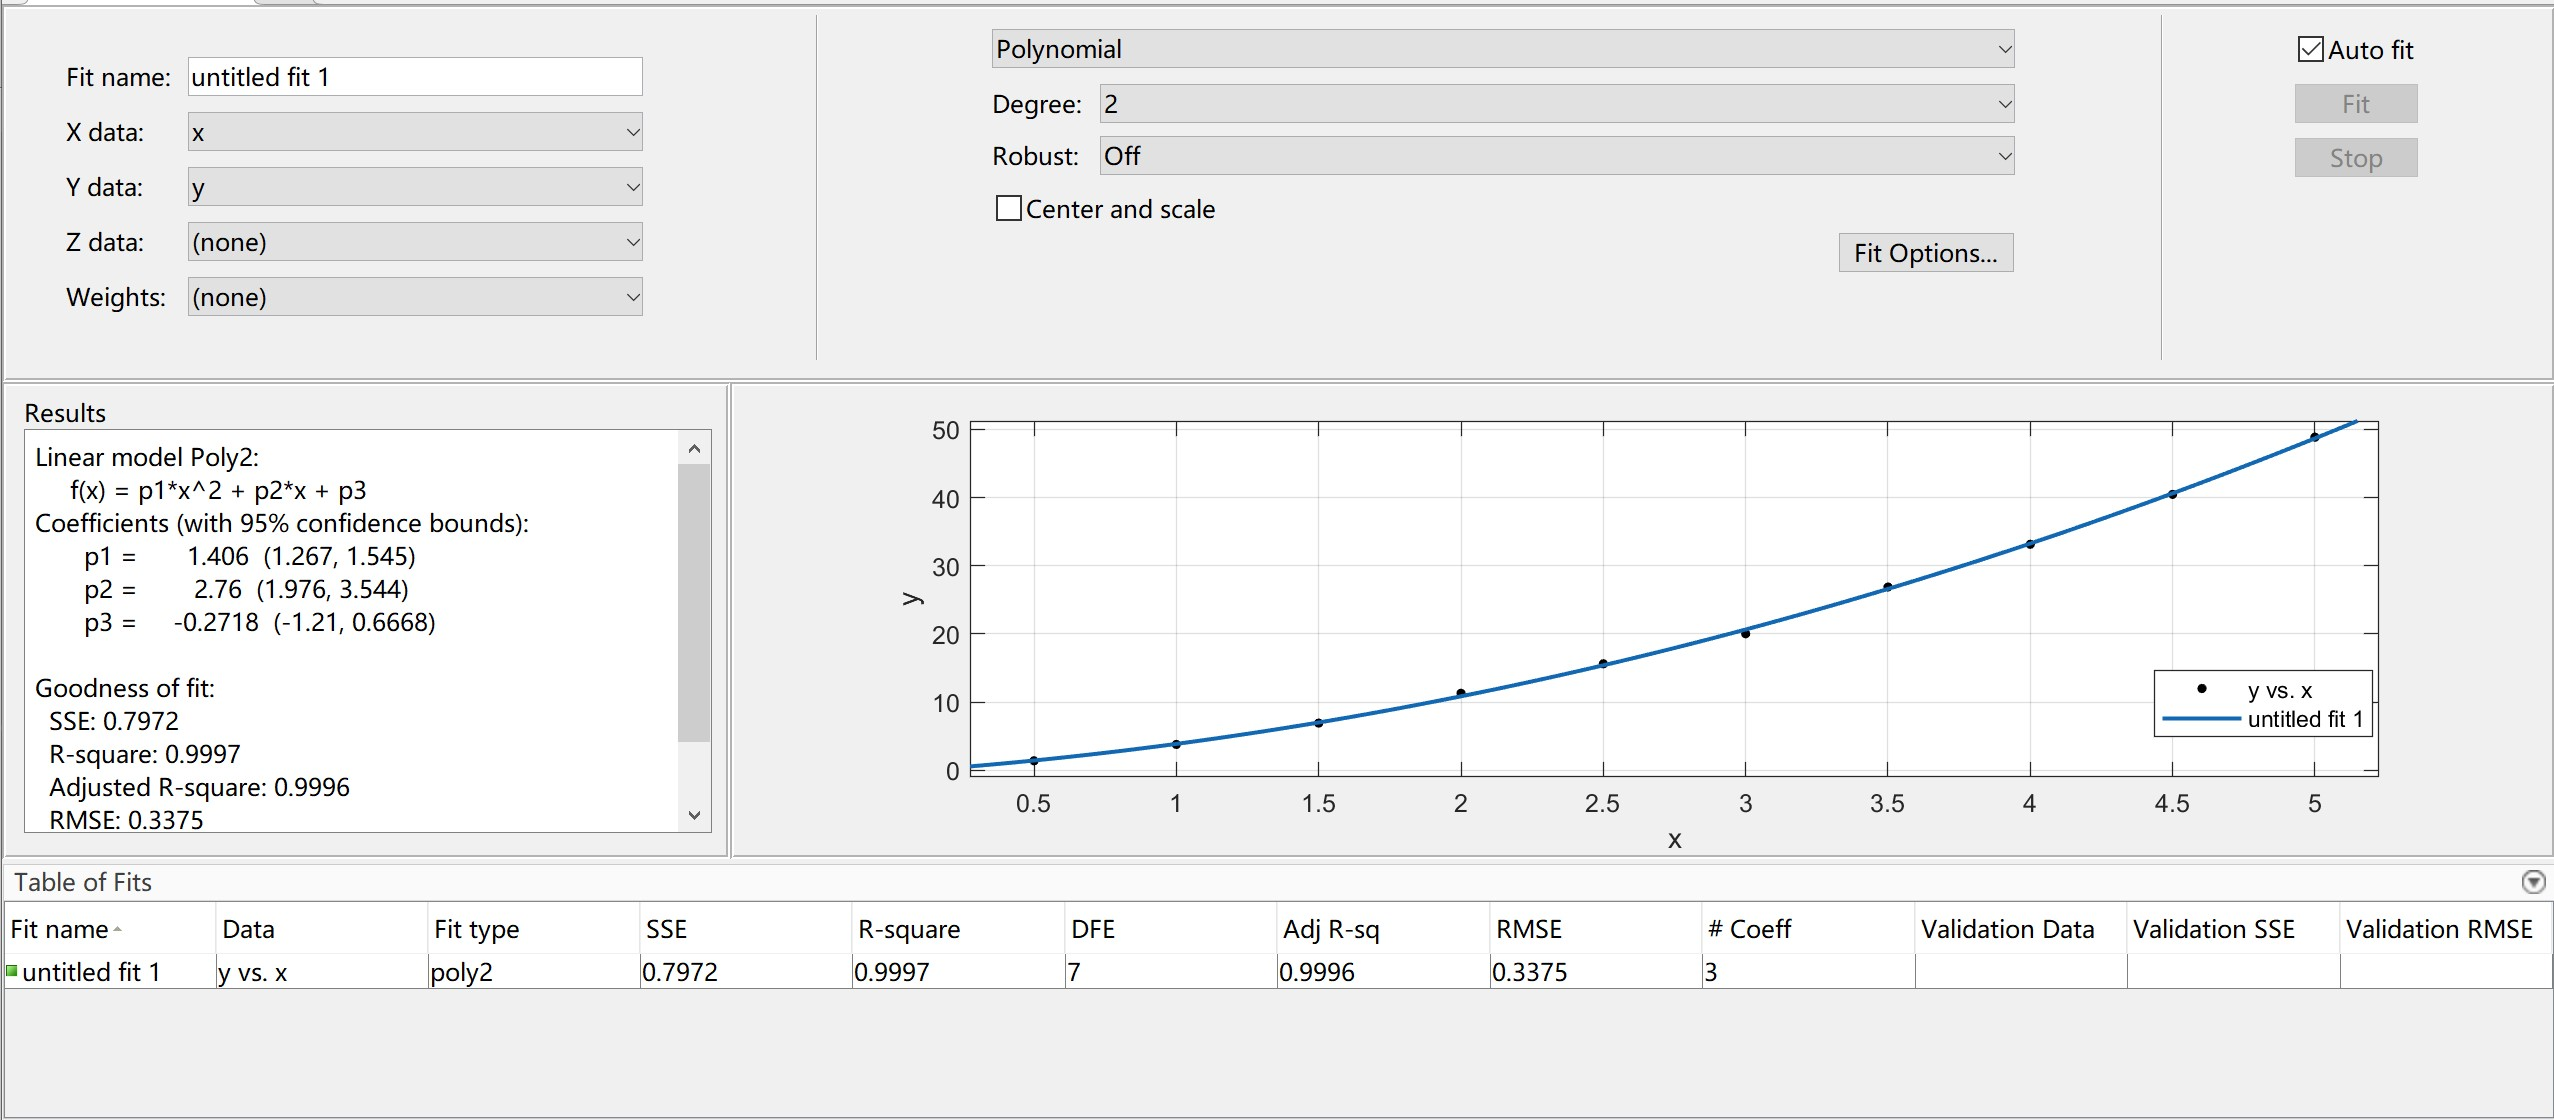
\includegraphics[width=0.6\textwidth,height=0.3\textwidth]{ex12_2_1.jpg}
        \caption{fitting result}
    \end{figure}\par
    We can directly read off the result: $b_2=1.406, b_1=2.76, b_0=-0.2718$. \par
    We can also get: $SS_{E}=0.7972, R^2=0.9997$.
\end{frame}

\begin{frame}
    \frametitle{ex 12.2 answer}
    Method 2: Direct calculation.
    \par
    \begin{figure}[H]
        \centering
        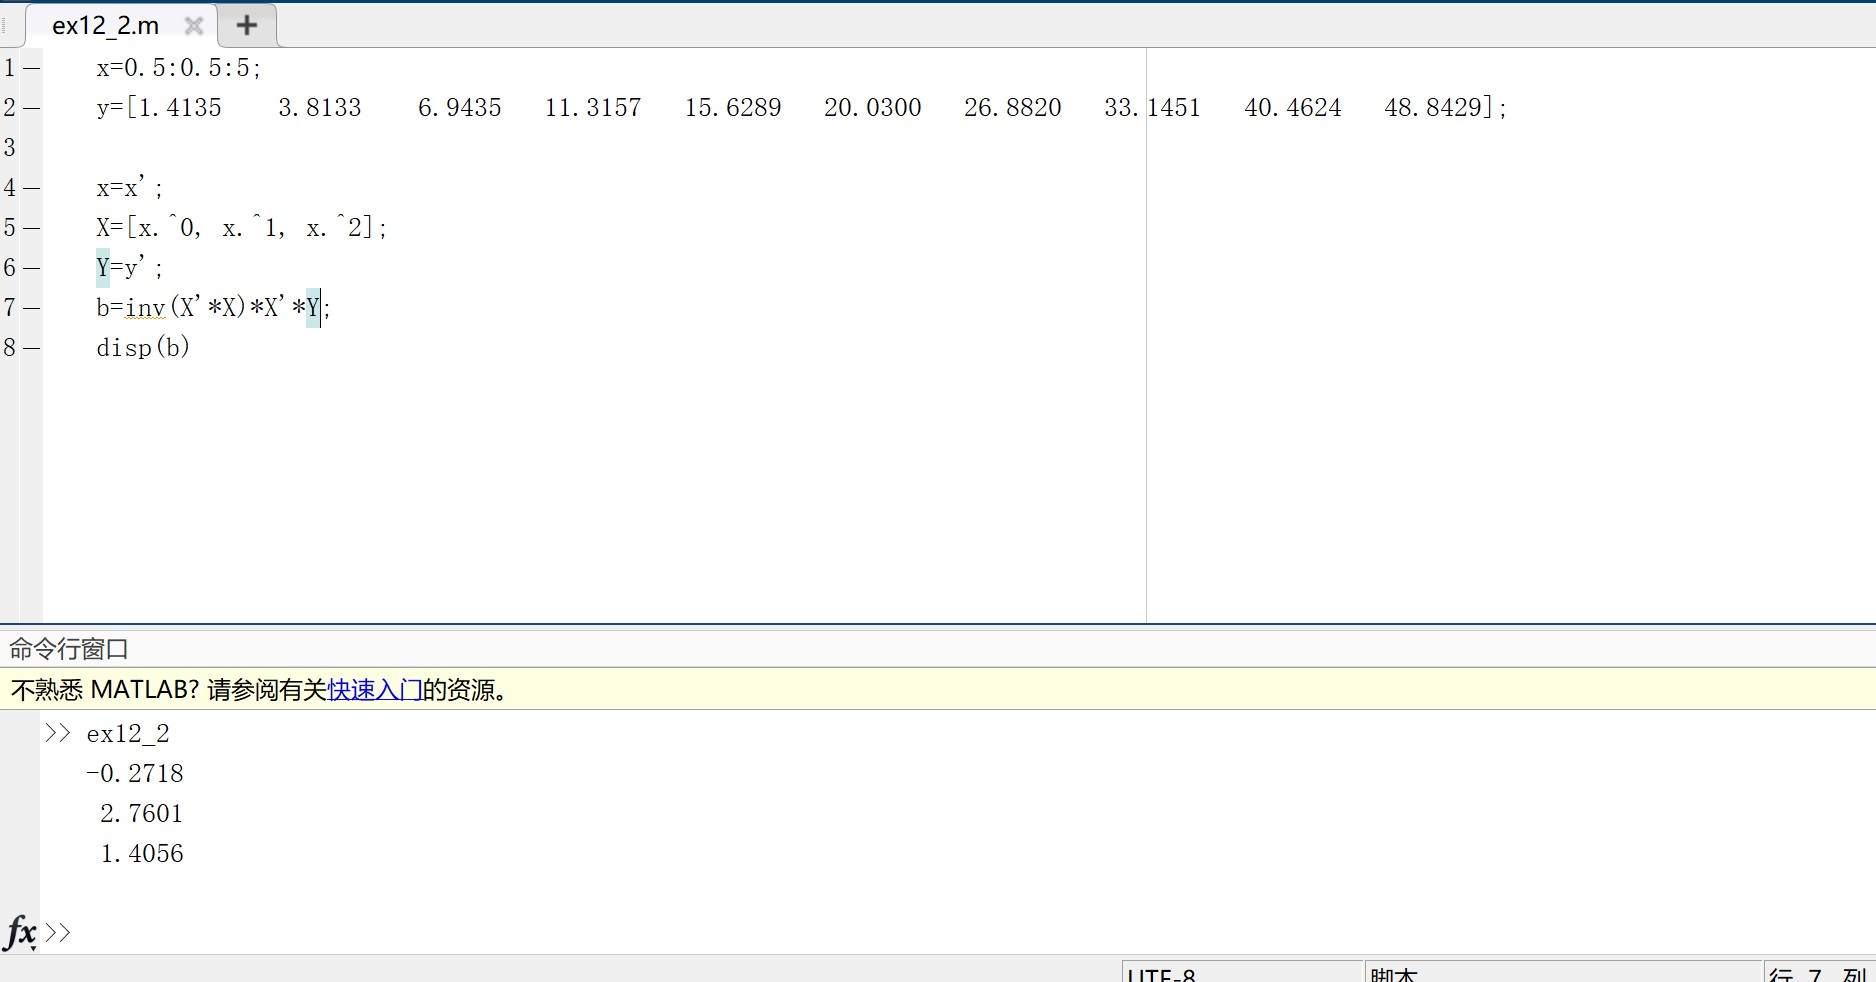
\includegraphics[width=0.6\textwidth,height=0.3\textwidth]{ex12_2_2.jpg}
        \caption{fitting result}
    \end{figure}\par
    We get basically the same result: $b_0=-0.2718, b_1=2.7601, b_2=1.4056$

\end{frame}

\begin{frame}
    \frametitle{The Multilinear Model}

    Basically the same thing. You need to use a different model specification matrix, which is
    \begin{equation*}
        X=
        \left(
        \begin{array}{ccccc}
            1 & x_{11} & x_{21} & \cdots & x_{p1}\\
            \vdots & \vdots & \vdots & \ddots & \vdots\\
            1 & x_{1n} & x_{2n} & \cdots & x_{pn}
        \end{array}
        \right)
    \end{equation*}
    And you can follow the same process.\par
    \textbf{note:} The matlab curve fitting tool can deal with up 2 free variables.

\end{frame}

\begin{frame}
    \frametitle{Error Analysis}

    We want to measure $SS_{E}$ and $R^2$. You can of course get them from matlab, but you're recommended to also know how to calculate them directly.\par
    Like the simple linear regression, we need to analysis $SS_{T}$ and $SS_{E}$.
    \[SS_{T}=\sum\limits_{i=1}^{n}(Y_i-\overline{Y})^2, SS_{E}=||Y-Xb||^2\]


\end{frame}

\begin{frame}
    \frametitle{Error Analysis}

    The P projection is an $n*n$ matrix with value $\frac{1}{n}$ for each of the element. The hat matrix $H:=X(X^{T}X)^{-1}X^{T}$. Our result for $SS_{T}$ and $SS_{E}$ are:
    \[SS_{E}=\Braket{Y, (\mathbb{I}_{n}-H)Y}, \]
    \[SS_{T}=\Braket{Y,(\mathbb{I}_{n}-P)Y}=SS_{E}+SS_{R}\]
    \[R^2=1-\frac{SS_{E}}{SS_{T}}\]
    \textbf{Notice:} You shouldn't use mathematica to calculate $R^2$ in function "NonLinearModelFit". Mathematica will use corrected $R^2$ which is not taught in our course. However, matlab will give correct answer.
\end{frame}

\begin{frame}
    \frametitle{ex 12.3}

    Calculate the $SS_E$ and $R^2$ in ex 12.2

\end{frame}

\begin{frame}
    \frametitle{ex 12.3 answer}

    \begin{figure}[H]
        \centering
        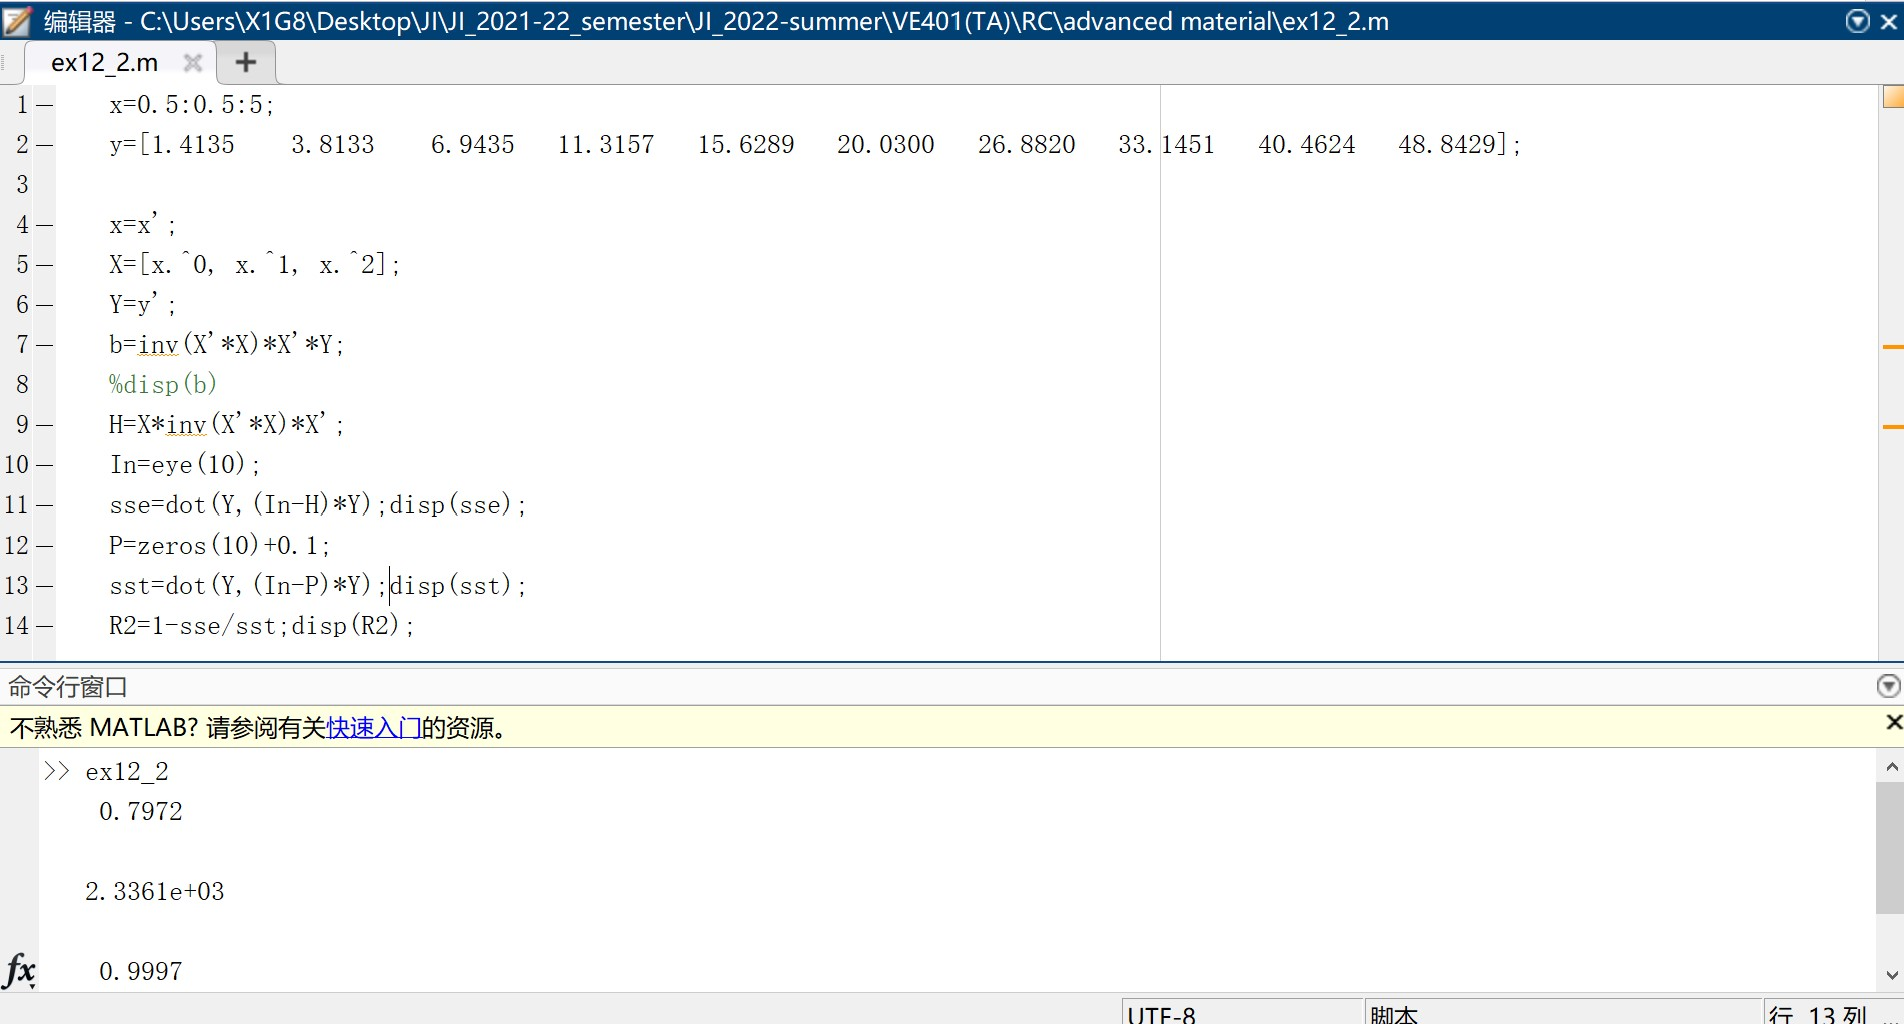
\includegraphics[width=0.6\textwidth,height=0.3\textwidth]{ex12_3.jpg}
        \caption{fitting result}
    \end{figure}\par
    The result is the same to ex12.2 when we use curve fitting toolbox: $SS_{E}=0.7972$, $R^2=0.9997$. Perfect!

\end{frame}

\section{Multiple Linear Regression II: Inferences on the Model}
\begin{frame}
    \frametitle{Outline}
    \tableofcontents[currentsection]
\end{frame}
\begin{frame}
    \frametitle{Distribution of the Sum of Squares Error}

    \[\frac{SS_E}{\sigma^2}=\Braket{Z,(1_n-H)Z}\quad(Z=(Z_1,Z_2,\dots , Z_n)^{T})\]
    And in practical,
    \[\frac{SS_E}{\sigma^2}\sim \chi^2_{n-p-1}\]
    $p$ is the number of variables in the regression model($x$ and $x^2$ term is counted as 2). $p+1$ is the number of terms. For example, for simple linear regression $p=1$ $(p+1=2)$, the model specification matrix has n rows and $(p+1)$ columns.\par
    Also, the estimator 
    \[S^2=\frac{SS_E}{n-p-1}\]
    is unbiased for $\sigma^2$

\end{frame}

\begin{frame}
    \frametitle{Significance of Regression}

    If there's no evidence that at least one of the regression coefficient (not constant term) is non-zero, the regression is called insignificant, otherwise called significant. \par
    We have learned 2 kind of test in simple linear regression. What are they? Which one do you think will be used here?

\end{frame}

\begin{frame}
    \frametitle{F-Test for Significance of Regression}
    The null hypothesis is $H_0: \beta_1=\beta_2=\dots  =\beta_p=0$\par
    The test statistic for the F-test is 
    \[F_{p,n-p-1}=\frac{SS_R/p}{S^2}=\frac{n-p-1}{p}\frac{R^2}{1-R^2}\]
    So you can easily determine the F statistic using only matlab. And it's a one-tailed test of course, so we reject $H_0$ at $F_{p,n-p-1}>f_{\alpha, p,n-p-1}$.\par


\end{frame}

\begin{frame}
    \frametitle{Analysis of the Parameters}
    What about T-test? T-test is used to determine the significance of a specified parameter. \par
    We need to analyze the variance of the estimator $B_0, B_1, \dots , B_p$.\par
    The result is, $Var[\textbf{b}]=\sigma^2(X^{T}X)^{-1}$. Denote $\xi_{ii}=((X^{T}X)^{-1})_{ii}$, we have 
    \[Var[B_i]=\xi_{ii}\sigma^2\]
    

\end{frame}

\begin{frame}
    \frametitle{Confidence Intervals for the Model Parameters}

    In practice, we use $S^2$ to estimate $\sigma^2$, so it'll be a T-test. The confidence interval for the parameter $\beta_j$ is
    \[b_j\pm t_{\alpha/2, n-p-1}S\sqrt{\xi_{jj}}\]
    for $j=0$ to $p$.
    We reject $H_0: \beta_j=0$ when 0 is not in the confidence interval of $\beta_j$.\par
    If the confidence(or significance) level is not specified by the question, you can always use a 95\% two-sided confidence interval, which can be directly read off from matlab. (You're still strongly recommended to write some step)

\end{frame}

\begin{frame}
    \frametitle{Confidence Intervals for the Estimated Mean}

    Short review question: What's the difference between confidence interval and prediction interval?\par
    \vspace{0.3cm}

    A $100(1-\alpha)\%$ confidence interval for $\mu_{Y|x_0}$ is 
    \[\mu_{Y|x_0}=\hat{\mu}_{Y|x_0}\pm t_{\alpha/2, n-p-1} S \sqrt{\mathbf{x_0}^{T}(X^{T}X)^{-1}\mathbf{x_0}}\]
    Here, the $\mathbf{x_0}\in \mathbb{R}^{p+1}$\par

    A $100(1-\alpha)\%$ prediction interval for $Y|x_0$ is 
    \[Y|x_0=\widehat{Y|x_0}\pm t_{\alpha/2, n-p-1} S \sqrt{1+\mathbf{x_0}^{T}(X^{T}X)^{-1}\mathbf{x_0}}\]
    Note that $\hat{\mu}_{Y|x_0}=\widehat{Y|x_0}$ is just $X\mathbf{b}$

\end{frame}

\begin{frame}
    \frametitle{Partial F-Test for Model Sufficiency}

    Some times a reduced model is good enough compared with full model. That is to say, $SS_{E,reduced}$ is not much bigger than $SS_{E, full}$.\par
    We set $H_0: \text{the reduced model is sufficient}$. We reject $H_0$ if there's evidence that $SS_{E,full}\ll SS_{E,reduced}$.\par
    \vspace{0.3cm}
    Now suppose that we have a full model of $p+1$ predictor variables, and a reduced model with $m+1$ ($m<p$) predictor variables.\par
    \vspace{0.3cm}
    The test statistic is $F_{p-m,n-p-1}=\frac{n-p-1}{p-m}\frac{SS_{E,reduced}-SS_{E,full}}{SS_{E,full}}$. Again this must be a one-tailed test, so we reject $H_0$ at significance level $\alpha$ if $F_{p-m,n-p-1}>f_{\alpha,p-m,n-p-1}$.\par
    \vspace{0.3cm}
    Partial F-test is actually the generalization of both T-test(for the significance of a single parameter) and F-test (for the significance of the whole model).

\end{frame}

\begin{frame}
    \frametitle{ex 12.4}

    We get a set of data:\par
    X: 1  2  3  4  5  6  7  8  9 10 \par
    Y: 2.23285627   7.36876551  14.59588823  24.8637199   37.73123178 54.3110869   74.2783259   95.9795571  120.28855899 148.37991283\par
    Please perform a linear regression with the model $\mu_{Y|x}=\beta_0+\beta_1 x+\beta_2 x^2$ and $\mu_{Y|x}=\beta_1 x+\beta_2 x^2$ respectively. Is $\beta_0$ necessary?

\end{frame}

\begin{frame}
    \frametitle{ex 12.4 answer}

    First perform a linear regression to the full model.
    \begin{figure}[H]
        \centering
        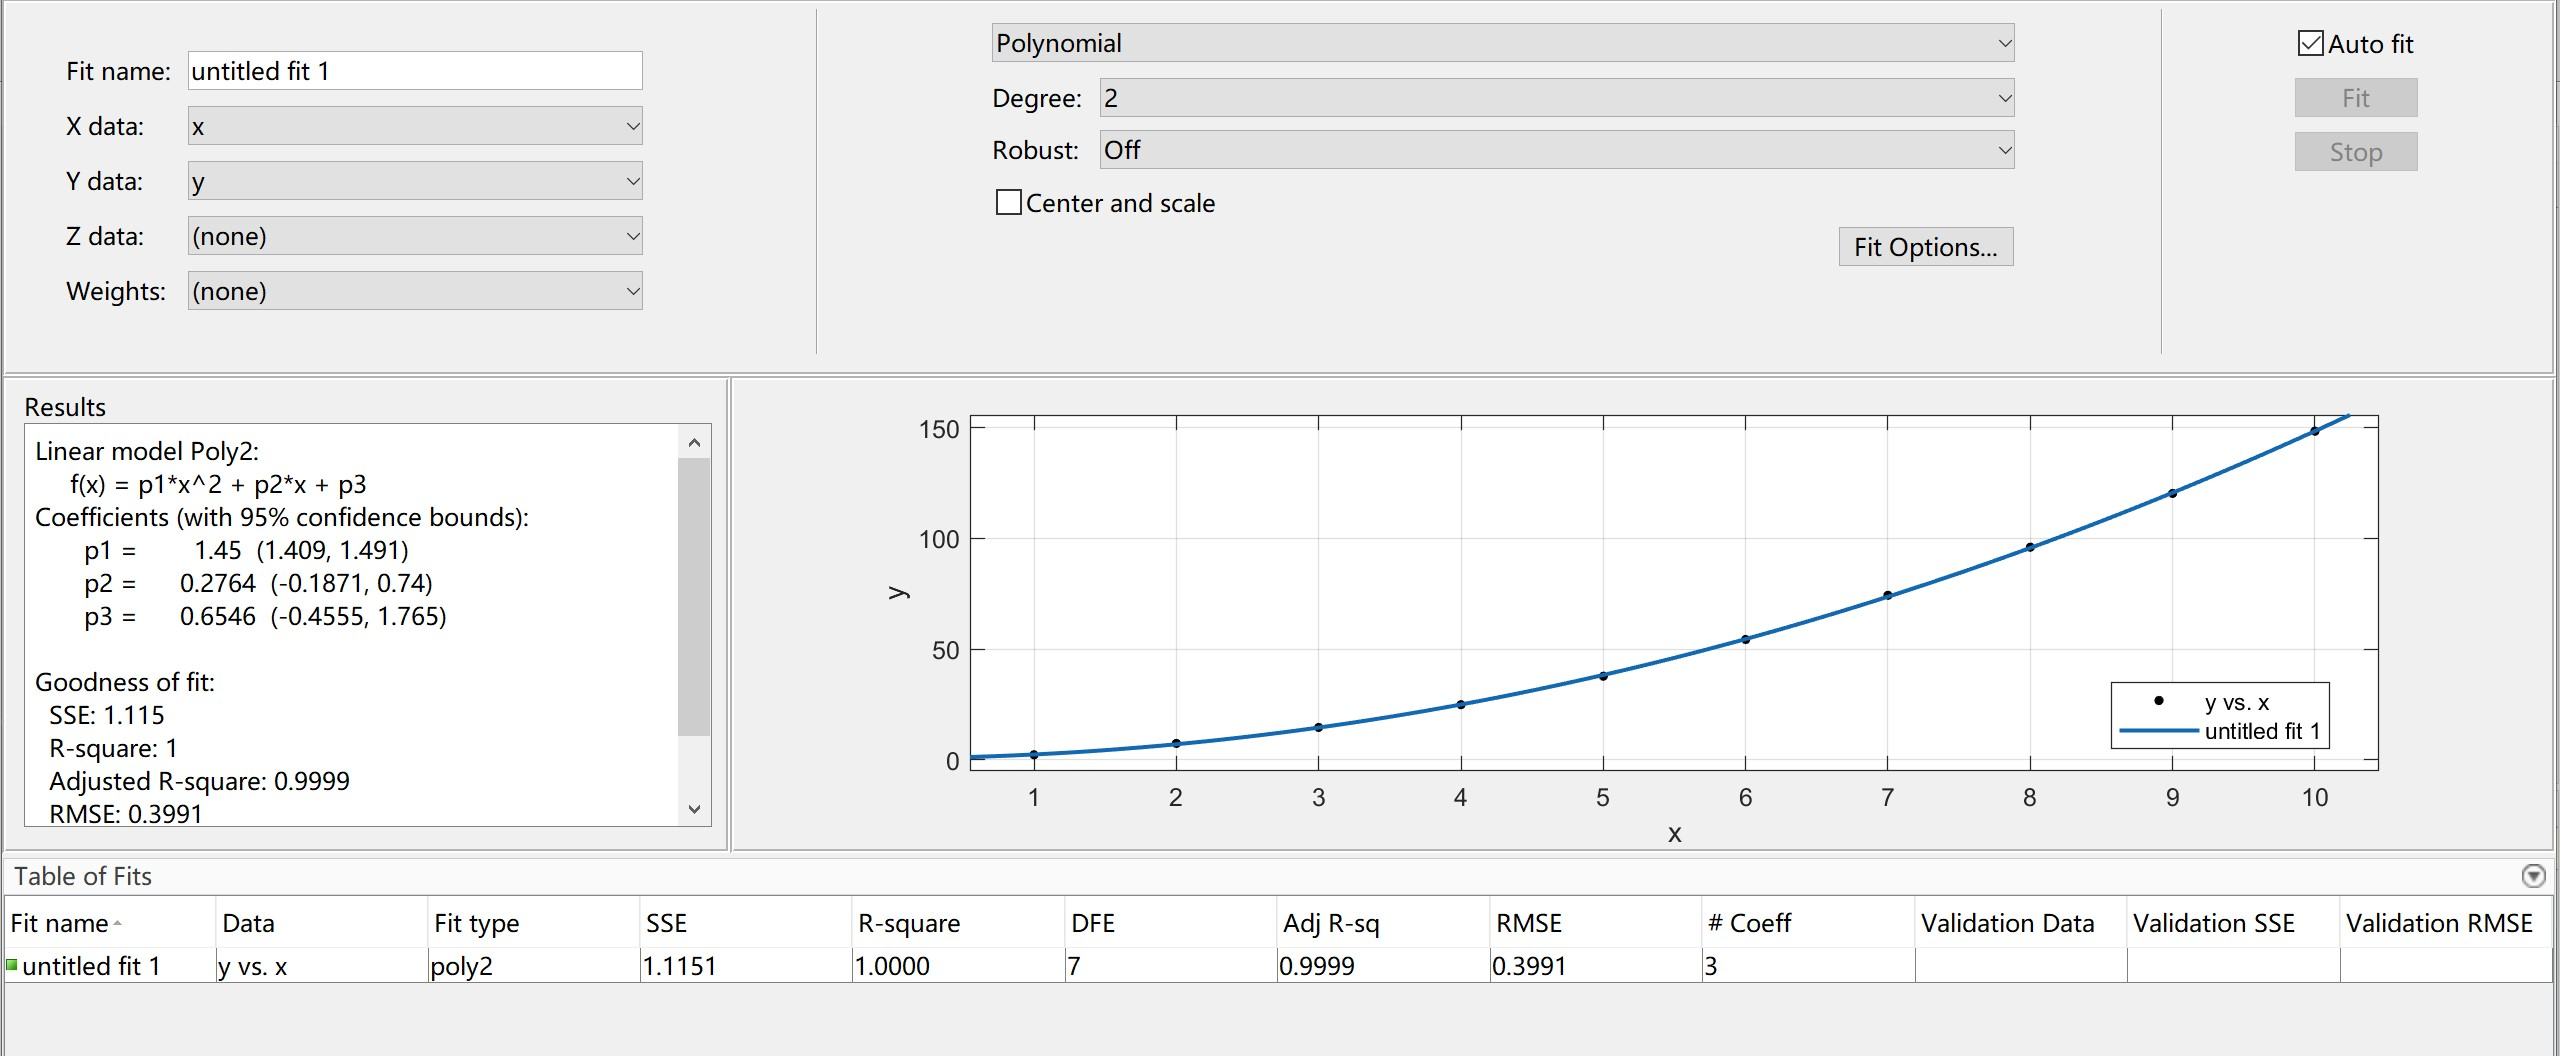
\includegraphics[width=0.6\textwidth,height=0.3\textwidth]{ex12_4_1.jpg}
        \caption{fitting result}
    \end{figure}\par
    The result is: $\beta_0=0.6546, \beta_1=0.2764, \beta_2=1.45$. $SS_E=1.115$

\end{frame}

\begin{frame}
    \frametitle{ex 12.4 answer}

    Next let's see the model without $\beta_0$.\par
    \begin{figure}[H]
        \centering
        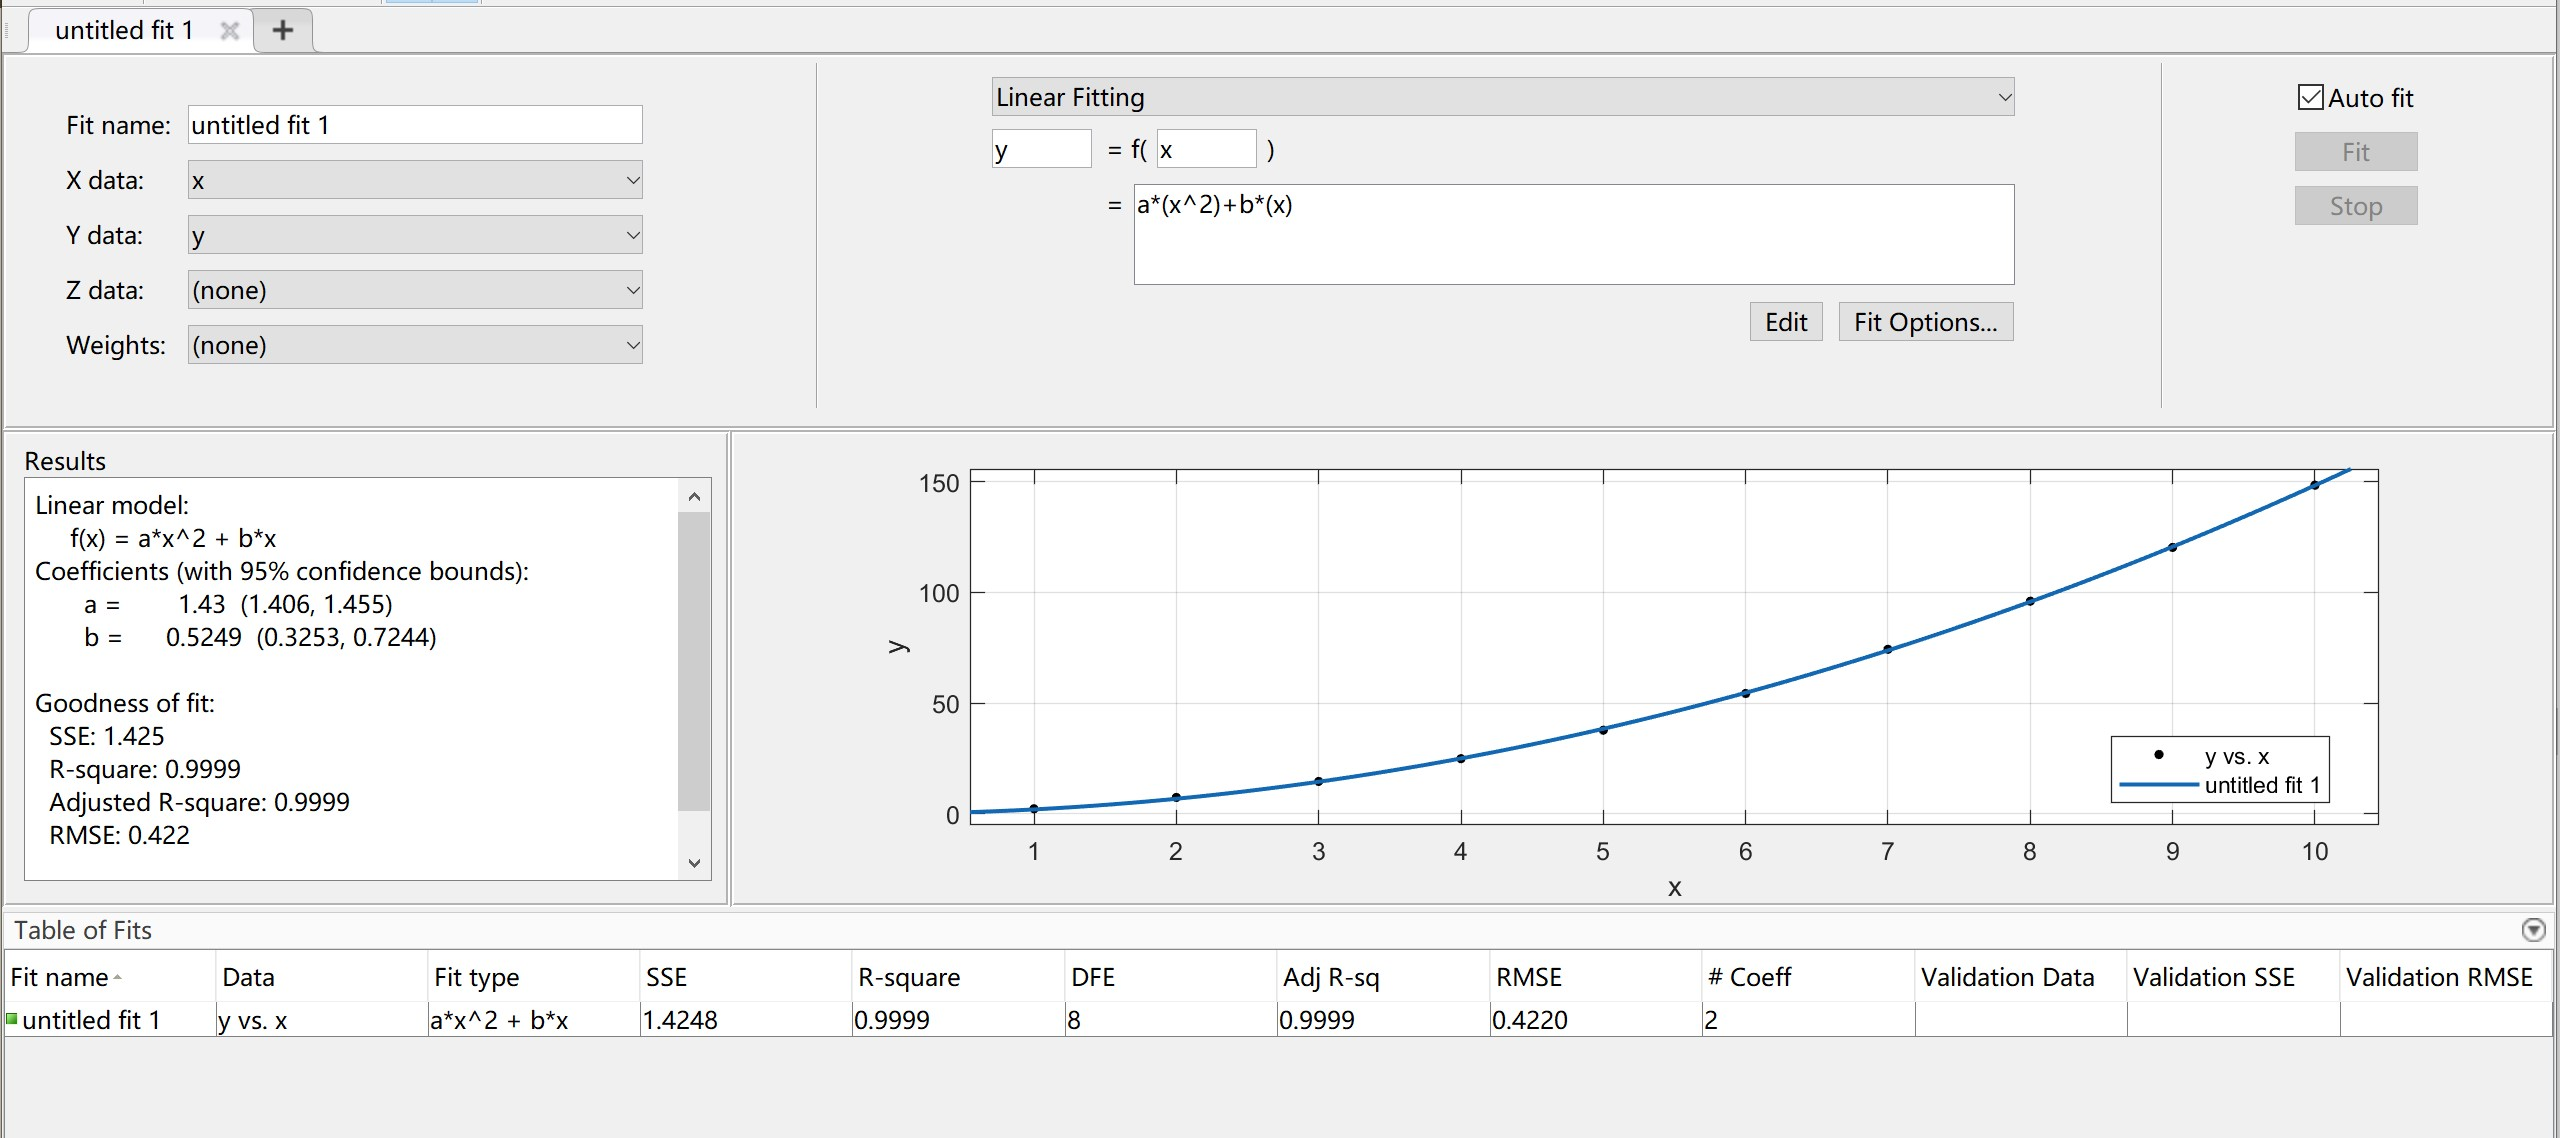
\includegraphics[width=0.6\textwidth,height=0.3\textwidth]{ex12_4_2.jpg}
        \caption{fitting result}
    \end{figure}\par
    The result is $\beta_1=0.5249, \beta_2=1.43$. $SS_E=1.425$\par
    Since the confidence interval of $\beta_0$ contains 0, our conclusion is that $\beta_0$ is not necessary.

\end{frame}

\section{Multiple Linear Regression III:
Finding the Right Model}
\begin{frame}
    \frametitle{Outline}
    \tableofcontents[currentsection]
\end{frame}

\begin{frame}
    \frametitle{Qualitative Predictors}

    \textbf{problem}: Include categorical predictors in a regression: brand, type,
    gender, etc.\par
    Method: introduce indicator variable $X$. $X=1$ means type A, and $X=0$ means type B.\par
    If there're more than 2 categories, for example, $k$ categories, then we need to introduce $k-1$ indicator variables. All zero means type 1, and $X_{m-1}=1$ means type m.\par
    \vspace{0.3cm}
    \textbf{example}: Suppose the solvent evaporation in spray paint is determined by humidity $x_1$ and paint brand A, B, C. The regression model is 
    \[\mu_{Y|x_1 x_2 x_3}=\beta_0+\beta_1 x_1+\beta_2 x_2+\beta_3 x_3\]
    And we have 
    \begin{equation*}
        (x_2,x_3)=\left\{
        \begin{aligned}
        (0,0) & : & \text{type A} \\
        (1,0) & : & \text{type B} \\
        (0,1) & : & \text{type C}
        \end{aligned}
        \right.
        \end{equation*}

\end{frame}

\begin{frame}
    \frametitle{Indicator Variables for Slope and Intercept}

    In the last example we actually suppose that the type has nothing to do with $\beta_1$. \par
    However it may not be the case. Now, for the two-type situation, we can make the model be
    \[\mu_{Y|x_1 x_2}=\beta_0+\beta_1 x_1+\beta_2 x_2 +\beta_3 x_1 x_2\]
    And we can use the model specification matrix in ex 12.1 to solve this problem.

\end{frame}

\begin{frame}
    \frametitle{ex 12.5}

    Suppose the solvent evaporation $Y$ in spray paint is determined by humidity $x_1$ and paint brand A, B. Also, the the brand will have influence on the coefficient of $X_1$. Please determine the model. The data is shown below:\par
    X: 1  2  3  4  5  6  7  8  9 10\par
    $Y_A$: 1.83041012  3.51241447  4.16901444  5.52485112  6.8984248   7.29818292
    9.5654521   9.27844592 11.63371656 11.95194421\par
    $Y_B$: 2.15060514  3.33394888  4.30853904  4.37507942  6.02694871  7.40665134
    8.2546196   9.77753879 11.66418639 11.4209547\par
    Is there evidence that the type has influence on the model?

\end{frame}

\begin{frame}
    \frametitle{ex 12.5 answer}

    We use the model $\mu_{Y|x_1 x_2}=\beta_0+\beta_1 x_1+\beta_2 x_2 +\beta_3 x_1 x_2$. Set type A: $x_2=1$ and type B: $x_2=0$.\par
    We can actually solve this problem with matlab.
    \begin{figure}[H]
        \centering
        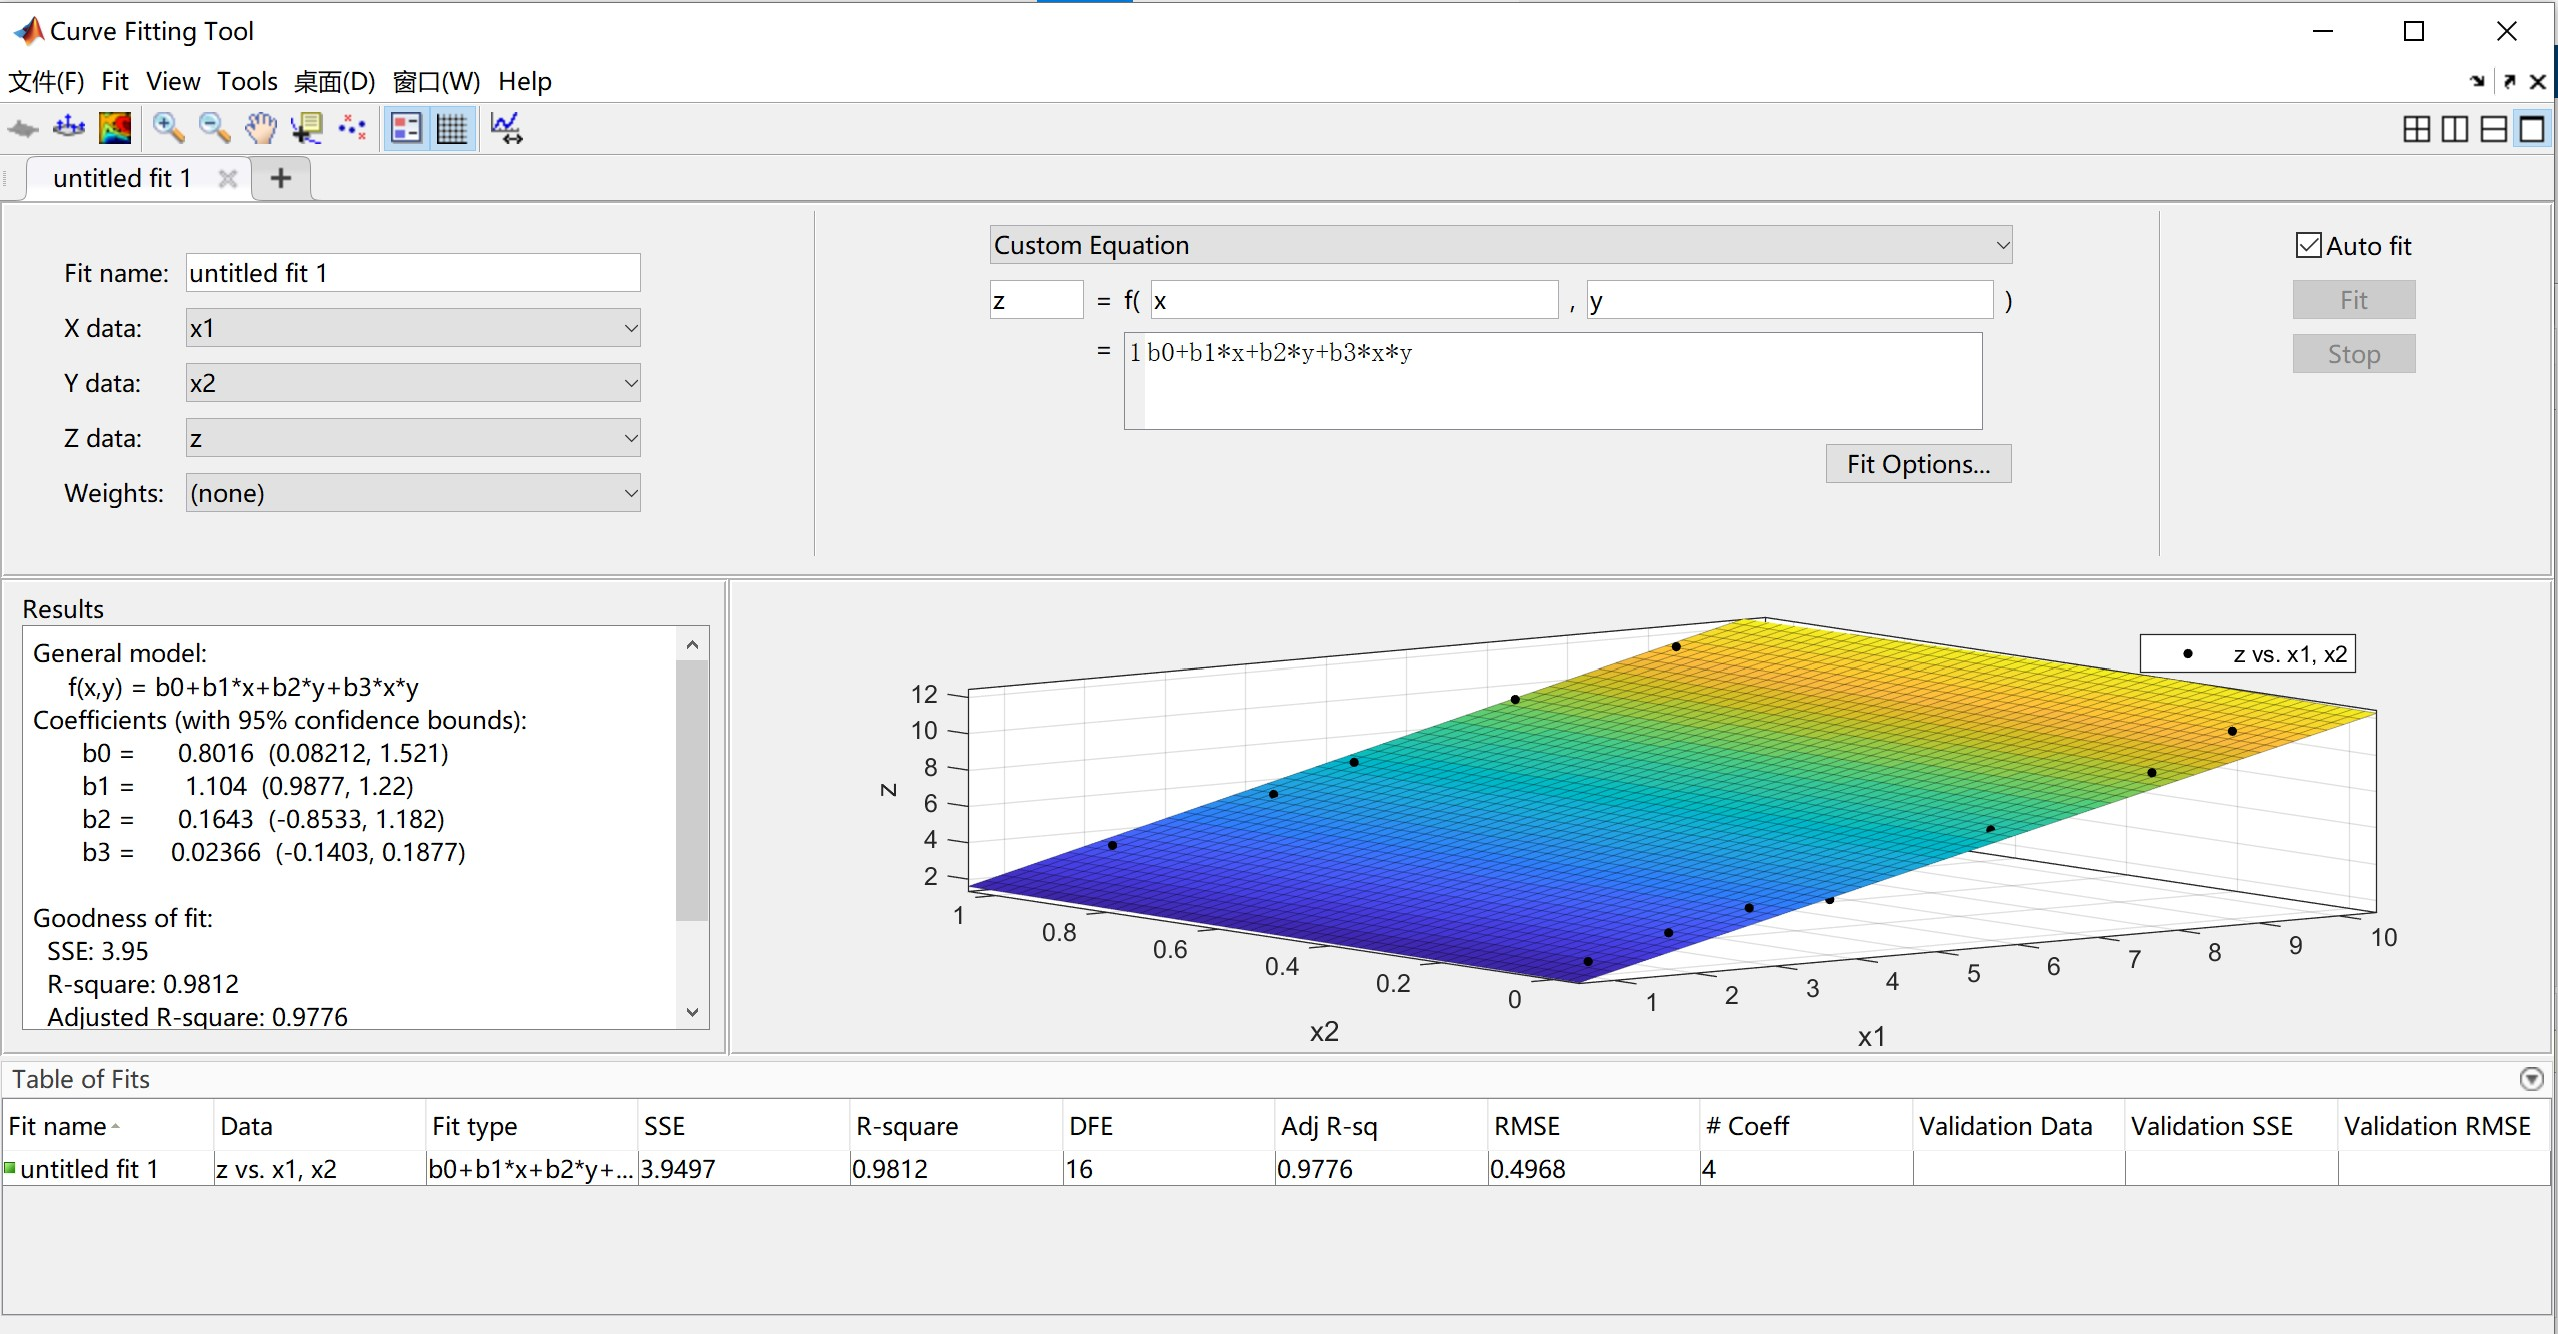
\includegraphics[width=0.56\textwidth,height=0.28\textwidth]{ex12_5.jpg}
        \caption{fitting result}
    \end{figure}\par
    The result is $\mu_{Y|x_1 x_2}=0.8016+1.104 x_1+0.1643 x_2 +0.024 x_1 x_2$.\par
    Question: 0 is included in the confidence interval of $\beta_2$ and $\beta_3$. Does that mean there's no influence of the type?
\end{frame}

\begin{frame}
    \frametitle{ex 12.5 answer}
    No! The software only give a confidence interval for the coefficients, which is not enough. We record the $SS_{E,full}=3.95$. Now, perform another test with only $x_1$ term.\par
    \begin{figure}[H]
        \centering
        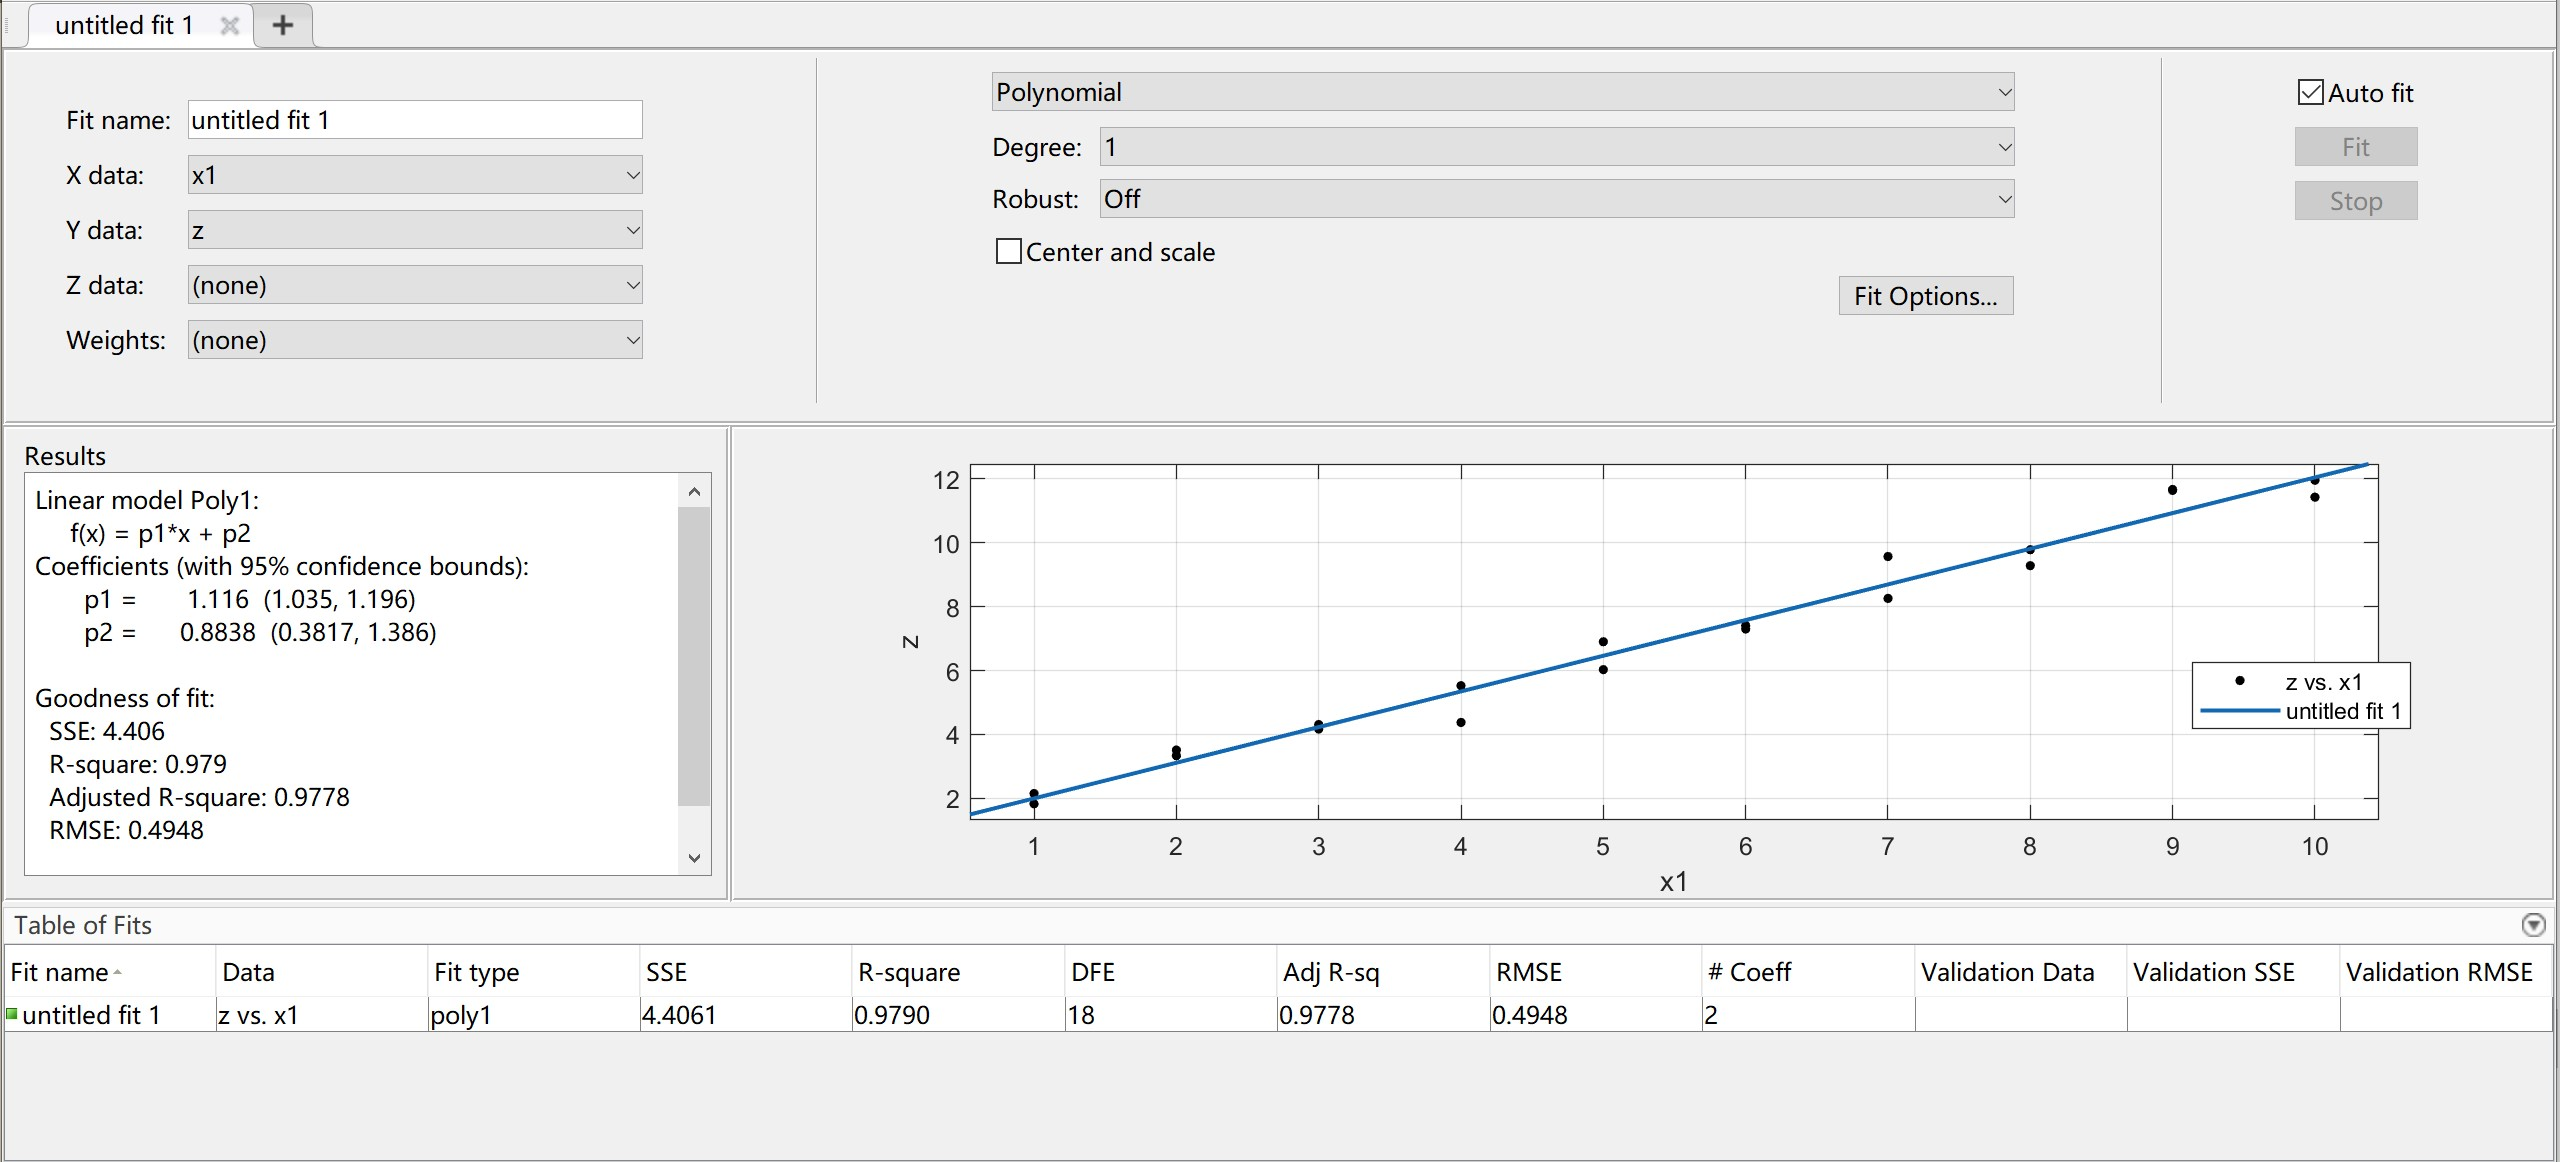
\includegraphics[width=0.5\textwidth,height=0.25\textwidth]{ex12_5_2.jpg}
        \caption{fitting result}
    \end{figure}\par
    We see that $SS_{E,reduced}=4.406$, so now we perform the partial-F test: n=20, p=3, m=1, so $F_{p-m,n-p-1}=F_{2,16}=0.924$. $f_{0.05,2,16}=3.63$, so we fail to reject $H_0:$ the reduced model is enough. Conclusion is, there's no evidence that the type influence $Y$.

\end{frame}

\begin{frame}
    \frametitle{Some other Exercise (if time permits)}

    

\end{frame}

\section{Conclusion and Q\&A}
\begin{frame}
    \frametitle{Outline}
    \tableofcontents[currentsection]
\end{frame}

\begin{frame}
    \frametitle{Conclusion of VE401}

    We finally get here!

\end{frame}

\begin{frame}
    \frametitle{OH Feedback (if time permits)}

    

\end{frame}

\begin{frame}
    \frametitle{ex 0.1 (In the Introduction RC 2 Month Ago ... )}
    What's your idea now?
    
    \begin{itemize}
        \item What's ``probability" and ``statistics" based on the probability and statistics knowledge you have learnt in your life?
        \item Is there a mathematical definition for ``probability"?
        \item What's the purpose of statistics? How can it help us understand and transform the world?
        \item Does statistics theory belong to mathematics? Why?
    \end{itemize}
    
\end{frame}

\begin{frame}
    \frametitle{ex 0.1 answer}

    Maybe...The answer is changing?

\end{frame}

\begin{frame}
    \frametitle{ex 0.2}

    What's your idea now?
    \begin{itemize}
    \item In physics lab, we calcuate type-A uncertainty by calcuating the sample deviation $S$, and use formula $t_{n-1}\frac{S}{\sqrt{n}}$. Have you ever thought what's the principle behind the formula?(\st{I know you haven't. This course is so annoying.} But now you have survived this course and let's revisit these contents again).
    \item In COVID-19 Hong Kong epidemic(2022 Feb-April), research has shown that the death rate for people who don't get vaccined is 2.87\%, while 0.14\% for fully vaccined(2 doses) and 0.03\% for boosted. Does that really show vaccine is so powerful?
    \item In USA, before general election, there'll be polls. However, for many times we can find that the result is different from polls. What factors may contribute to the difference?
    \end{itemize}
    
\end{frame}

\begin{frame}
    \frametitle{ex 0.2 answer}

    \begin{itemize}
        \item Central limit theorem. The sum of many tiny errors follows a normal distribution approximately.
        \item Correlation does not imply causation. This indeed shows the vaccine is useful, but not necessarily so powerful. At that time there's actually not many elder people with underlying disease fully vaccined. However, they're the vulnerable population of COVID-19.
        \item Polls can be regarded as the sample of election with some error. If set $\alpha=0.05$, the percentage difference should be greater than
        $\frac{98\%}{\sqrt{n}}$
    \end{itemize}

\end{frame}

\begin{frame}
    \frametitle{Q\&A}
    See you in EECS 501 (Probability and Random Processes) this winter!\par
    Feel free to ask me any question in the OH.\par
    Cheers!

\end{frame}

\end{document} 